% TFG - José Ángel Martín Baos. Escuela Superior de Informática. 2018
%%%% CHAPTER: Installation Guide %%%
% !TeX spellcheck = en_GB

\chapter{Installation guide} % TODO: Revise all
\label{chap:installation_guide}

\drop{I}{n} this appendix, the steps to install and configure the Raspberry Pi device in order to execute the software developed in this project are explained. Raspbian \ac{OS} \cite{Raspbian} is the Operative System that will be installed on the Raspberry Pi. Raspbian is an modification of Debian \ac{OS} for Raspberry Pi and ARM processors. In this installation guide, a GNU/Linux Operating System has been employed in the personal computer.


\section{Installation and configuration of Raspbian}
The first step to get the device working consists in the installation of the Raspbian Operating System and the configuration of the device to allow us access the Raspberry from another device using a wireless connection.

\subsection{Installation of Raspbian in a SD card}
There are two main alternatives to install Raspbian in the Raspberry Pi. The first one consists in downloading the \ac{OS} image and extracting it into the SD card, which is the method explained here. The second form, which is recommended for people with lower knowledge on Linux \ac{OS}, consists in downloading the NOOBS software. This software has to be copied into the SD card and when the Raspberry Pi is executed for the first time an installation process will be carried out and Raspbian will be installed. 

Raspbian \ac{OS} can be downloaded from the Raspberry Pi downloads page\footnote{Raspbian download page: \url{https://www.raspberrypi.org/downloads/raspbian/}}. Once downloaded, the following steps should be followed in order to have Raspbian properly working on the Raspberry Pi board:
\begin{enumerate}
	\item Download Raspbian and check the download. To check if the download has been correctly carried out, the following command has to be executed, where \emph{file.zip} is the downloaded file and \emph{hash\_value} is the SHA-1 value for the downloaded file which can be found on the download page.
\begin{console}
$ sha1sum file.zip | grep hash_value
\end{console} %$

	\item Now, the mirco-SD card can be inserted and mounted on the computer. Usually the card gets mounted automatically. The list of devices mounted on the computer is shown in the Figure \ref{fig:Appendix_df-h_command}. Here, it can be observed that the mirco-SD card correspond to the route \texttt{/dev/sdb1}. The command used is: 
\begin{console}
$ df -h
\end{console} %$
	\begin{figure}[!h]
		\begin{center}
			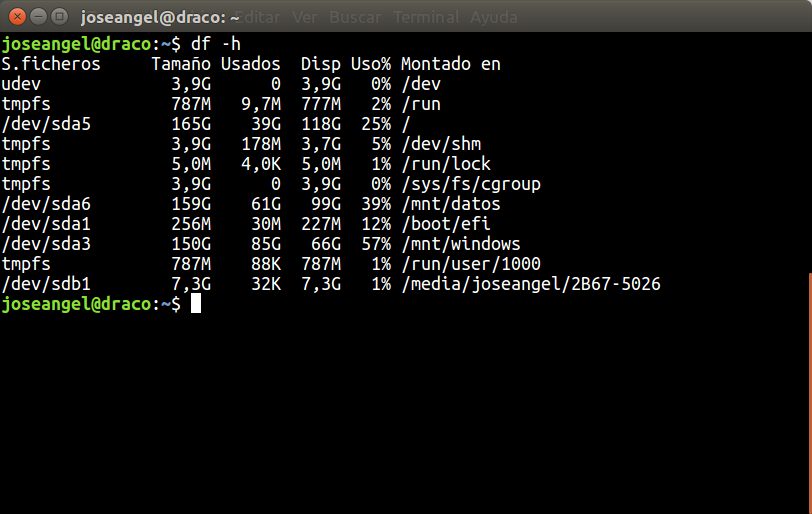
\includegraphics[width=0.9\textwidth]{Appendix_df-h_command.png}
			\caption{\texttt{df -h} command execution}
			\label{fig:Appendix_df-h_command}
		\end{center}
	\end{figure}

	\item Once the path where mirco-SD has been mounted is known, the next step is to execute the following command to unmount the card, where \texttt{/dev/sdb1} is de route corresponding to your card. This avoids that the \ac{OS} writes the card while the files are being copied.
\begin{console}
$ umount /dev/sdb1
\end{console} %$

	\item Now, the \ac{OS} image can be extracted and copied to the micro-SD card as shown in Figure \ref{fig:Appendix_SO_copy}. The following commands have to be executed from the directory where the file has been downloaded:
\begin{console}
$ unzip 2017-07-05-raspbian-jessie.zip 
$ sudo dd bs=4M if=2017-07-05-raspbian-jessie.img of=/dev/sdb1
\end{console} %$

	\begin{figure}[!h]
		\begin{center}
			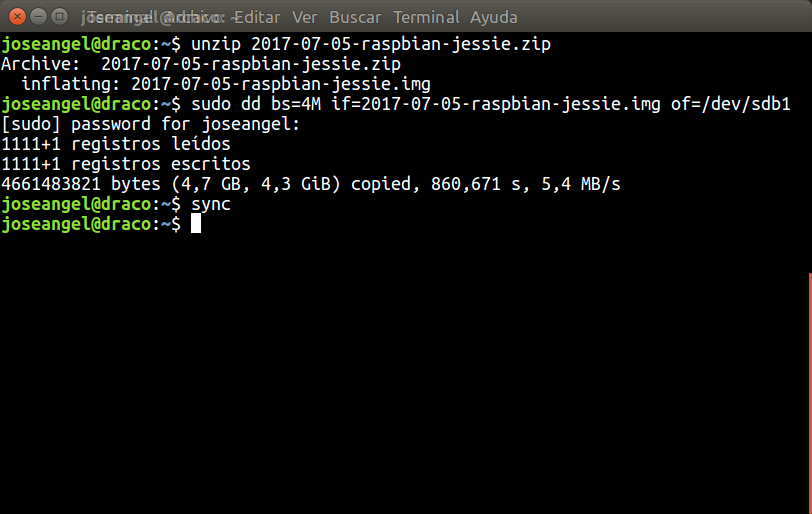
\includegraphics[width=0.9\textwidth]{Appendix_SO_copy.png}
			\caption{Console screenshot that shows the \ac{OS} copy process}
			\label{fig:Appendix_SO_copy}
		\end{center}
	\end{figure}

	\item Once the process has finished and before extracting the micro-SD card from the computer it should be ensured that the cache is clean. The next command must be executed:
\begin{console}
$ sync
\end{console} %$
	
\end{enumerate}


\subsection{Configuring Raspbian}
At this moment, the Raspbery Pi can be turned on. But firstly, it has to be connected to a external monitor or a TV using a HDMI cable. Nonetheless, this way is not very practical, therefore, some methods for allowing remote connection are explained. 

The first method consists in using \emph{ssh} protocol to access the Raspbery device. This protocol allows operating network services securely over an unsecured network. In others words, this method allows executing commands on the Raspberry Pi using a console, provided that the Raspberry Pi and the computer from where it is accessed are connected to the same network. OpenSSH tool \cite{OpenSsh} is installed with Raspbian \ac{OS} to provide the \emph{ssh} service. To activate it the following command should be executed:
\begin{console}
$ sudo raspi-config
\end{console} %$
This command executes the Raspbian configuration tool (Figure \ref{fig:Appendix_raspi-config_main}). \emph{Interfacing options} has to be selected. Using the new menu (Figure \ref{fig:Appendix_raspi-config_ssh}) SSH service should be selected and activated. Finally, the Raspberry Pi must be rebooted.

At this moment, the Raspberry Pi can be accessed from any computer connected to the same network using the next command, where \texttt{ipaddress} is the IP address of the network interface of the Raspberry Pi.
\begin{console}
$ ssh pi@ipaddress
\end{console} %$


The second method, consists in using a graphic remote session. VNC\footnote{VNC proyect main page: \url{http://www.hep.phy.cam.ac.uk/vnc_docs/index.html}} can be installed. VNC stands for Virtual Network Computing. It is, in essence, a remote display system which allows the user to view a computing 'desktop' environment, not only on the machine where it is running, but from anywhere on the Internet and from a wide variety of machine architectures. 

To activate VNC, the Interfacing options of the \texttt{raspi-config} tool has to be opened again as show in Figure \ref{fig:Appendix_raspi-config_ssh}. Then, VNC has to be selected and activated. Finally, the Raspberry Pi must be rebooted.

\begin{figure}[!h]
	\centering
	\subfigure[Main menu]{
		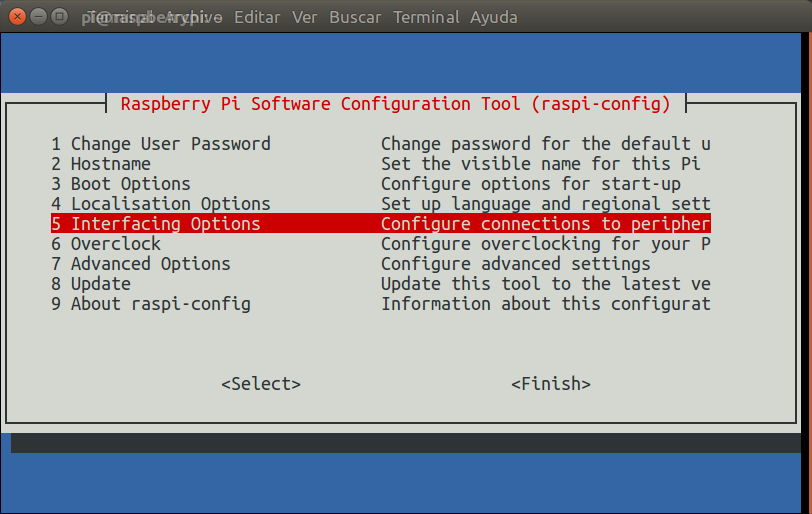
\includegraphics[width=0.48\textwidth]{Appendix_raspi-config.png}
		\label{fig:Appendix_raspi-config_main}
	}
	\subfigure[Interfacing Options]{
		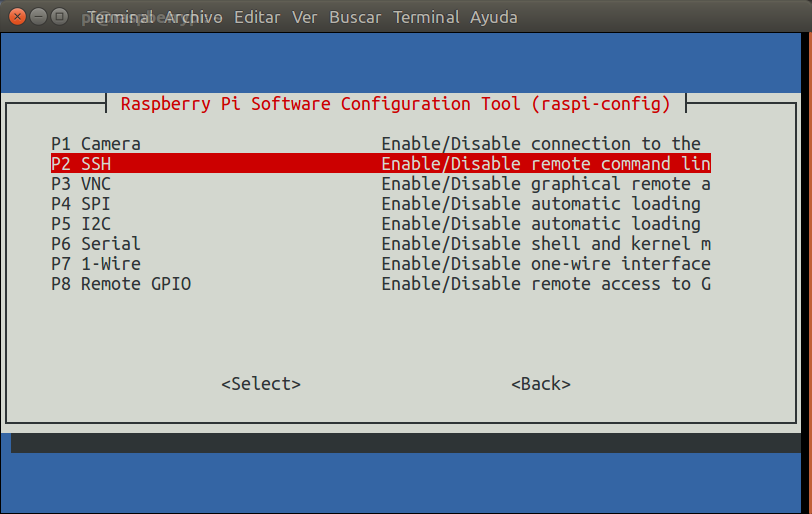
\includegraphics[width=0.48\textwidth]{Appendix_raspi-config_ssh.png}
		\label{fig:Appendix_raspi-config_ssh}
	}
	\caption{Screenshot of raspi-config tool}
	\label{fig:Appendix_raspi-config}
\end{figure}

To access the \textsc{vnc} server executing in the Raspberry Pi, we have opted for using \textsc{vnc} viewer for Google Chrome, which is a version of \textsc{vnc} Connect\footnote{RealVNC main page: \url{https://www.realvnc.com/en/}} application adapted to execute in Google Chrome web browser. A screenshot of the program can be shown in Figure \ref{fig:Appendix_VNC-Viewer-Chrome}.

\begin{figure}[!h]
	\begin{center}
		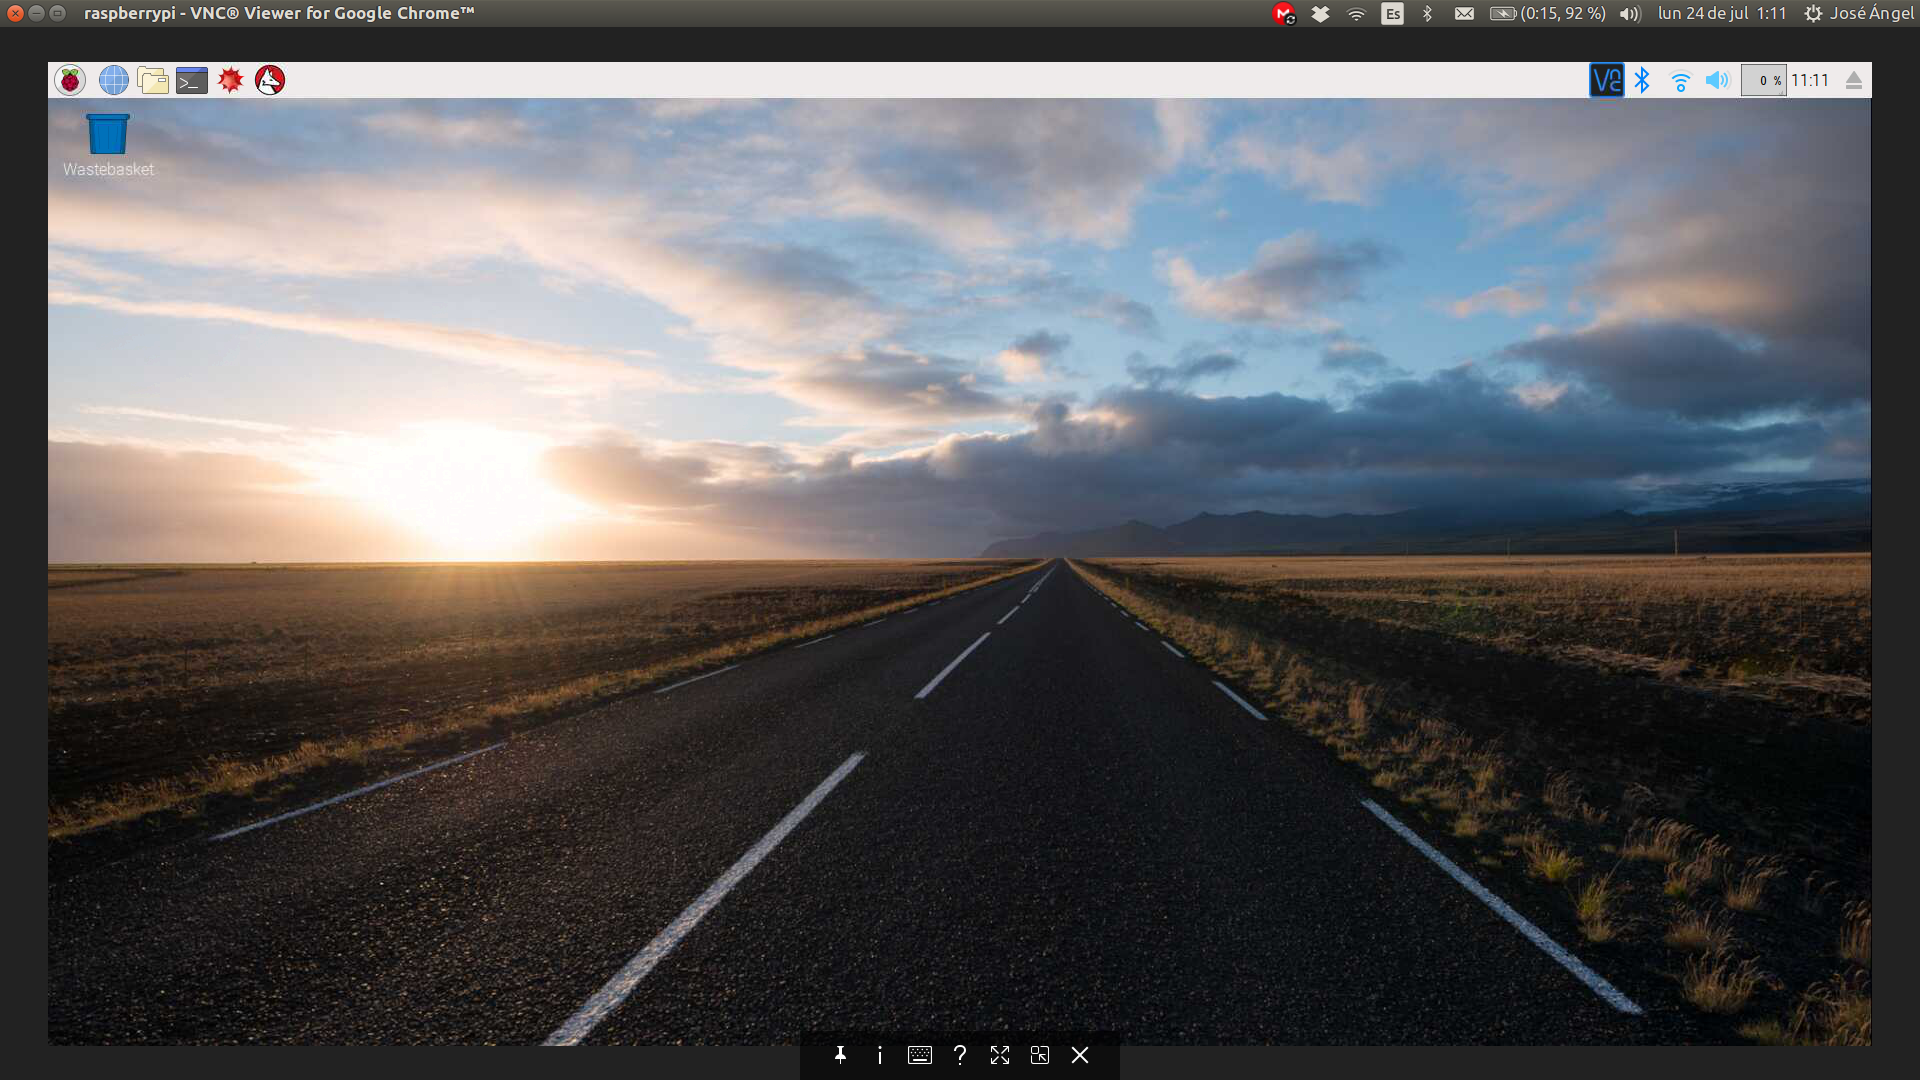
\includegraphics[width=1\textwidth]{Appendix_VNC-Viewer-Chrome.png}
		\caption{Screenshot of \textsc{vnc} Viewer for Google Chrome.}
		\label{fig:Appendix_VNC-Viewer-Chrome}
	\end{center}
\end{figure}

The last step in this configuration process is to update the Raspbian \ac{OS} and applications. To accomplish this task, first, the filesystem should be expanded. This means that all the free space in the SD card will be available to the \ac{OS}. Again, the raspberry configuration tool has to be executed (Figure \ref{fig:Appendix_raspi-config_main}), and the \emph{Advance Options} menu has to be opened. Then, the \emph{Expand Filesystem} option must be selected. To finish with, the following commands have to be executed to update Rasbian:
\begin{console}
$ sudo apt-get update
$ sudo apt-get upgrade
\end{console} %$


\section{Installation of the necessary hardware and software}
Once we have the Raspberry Pi configured, it is needed to install some basic software and configure the hardware. In this case, as Python 3 had been used to develop the program that runs into the Raspberry Pi, Python 3 package installer (known as PIP) is needed. This software allows to install Python 3 packages easily. The next command has to be executed:
\begin{console}
$ sudo apt-get install python3-pip
\end{console} %$

\subsection{Installation of the PiCamera module}
In this project, the \emph{Raspberry Pi camera module V2} \footnote{More information about the Raspberry Pi camera module can be found in: \url{https://www.raspberrypi.org/products/camera-module-v2/}} is used. PiCamera \cite{PiCameraDoc} library is used to manage the Raspberry Pi camera installed. This library can be found on the Raspbian repositories, so it can be installed easily using the \emph{apt-get} command:
\begin{console}
$ sudo apt-get install python3-picamera
\end{console} %$

The next step is to enable the camera connection. The raspberry configuration tool will be executed (Figure \ref{fig:Appendix_raspi-config_main}), and the \emph{Interfacing options} menu should be opened. There, \emph{Camera} must be selected and activated. Then, the system should be restarted. Is important to know that the camera may not work well if there is not at least 128 MB of memory asignated to the \textsc{gpu}.

The last step is to connect the camera to the Raspbery Pi. The \textsc{csi} port must be used for this purpose. This port is located between the \textsc{hdmi} port and the stereo plug. It is advisable that when the camera is being installed the Raspberry must be turned off to avoid any damage to the camera. When connecting it, the blue part of the bus must be facing the stereo plug and the Ethernet connection as it is shown in Figure \ref{fig:Appendix_camera_conection}. 

\begin{figure}[!h]
	\begin{center}
		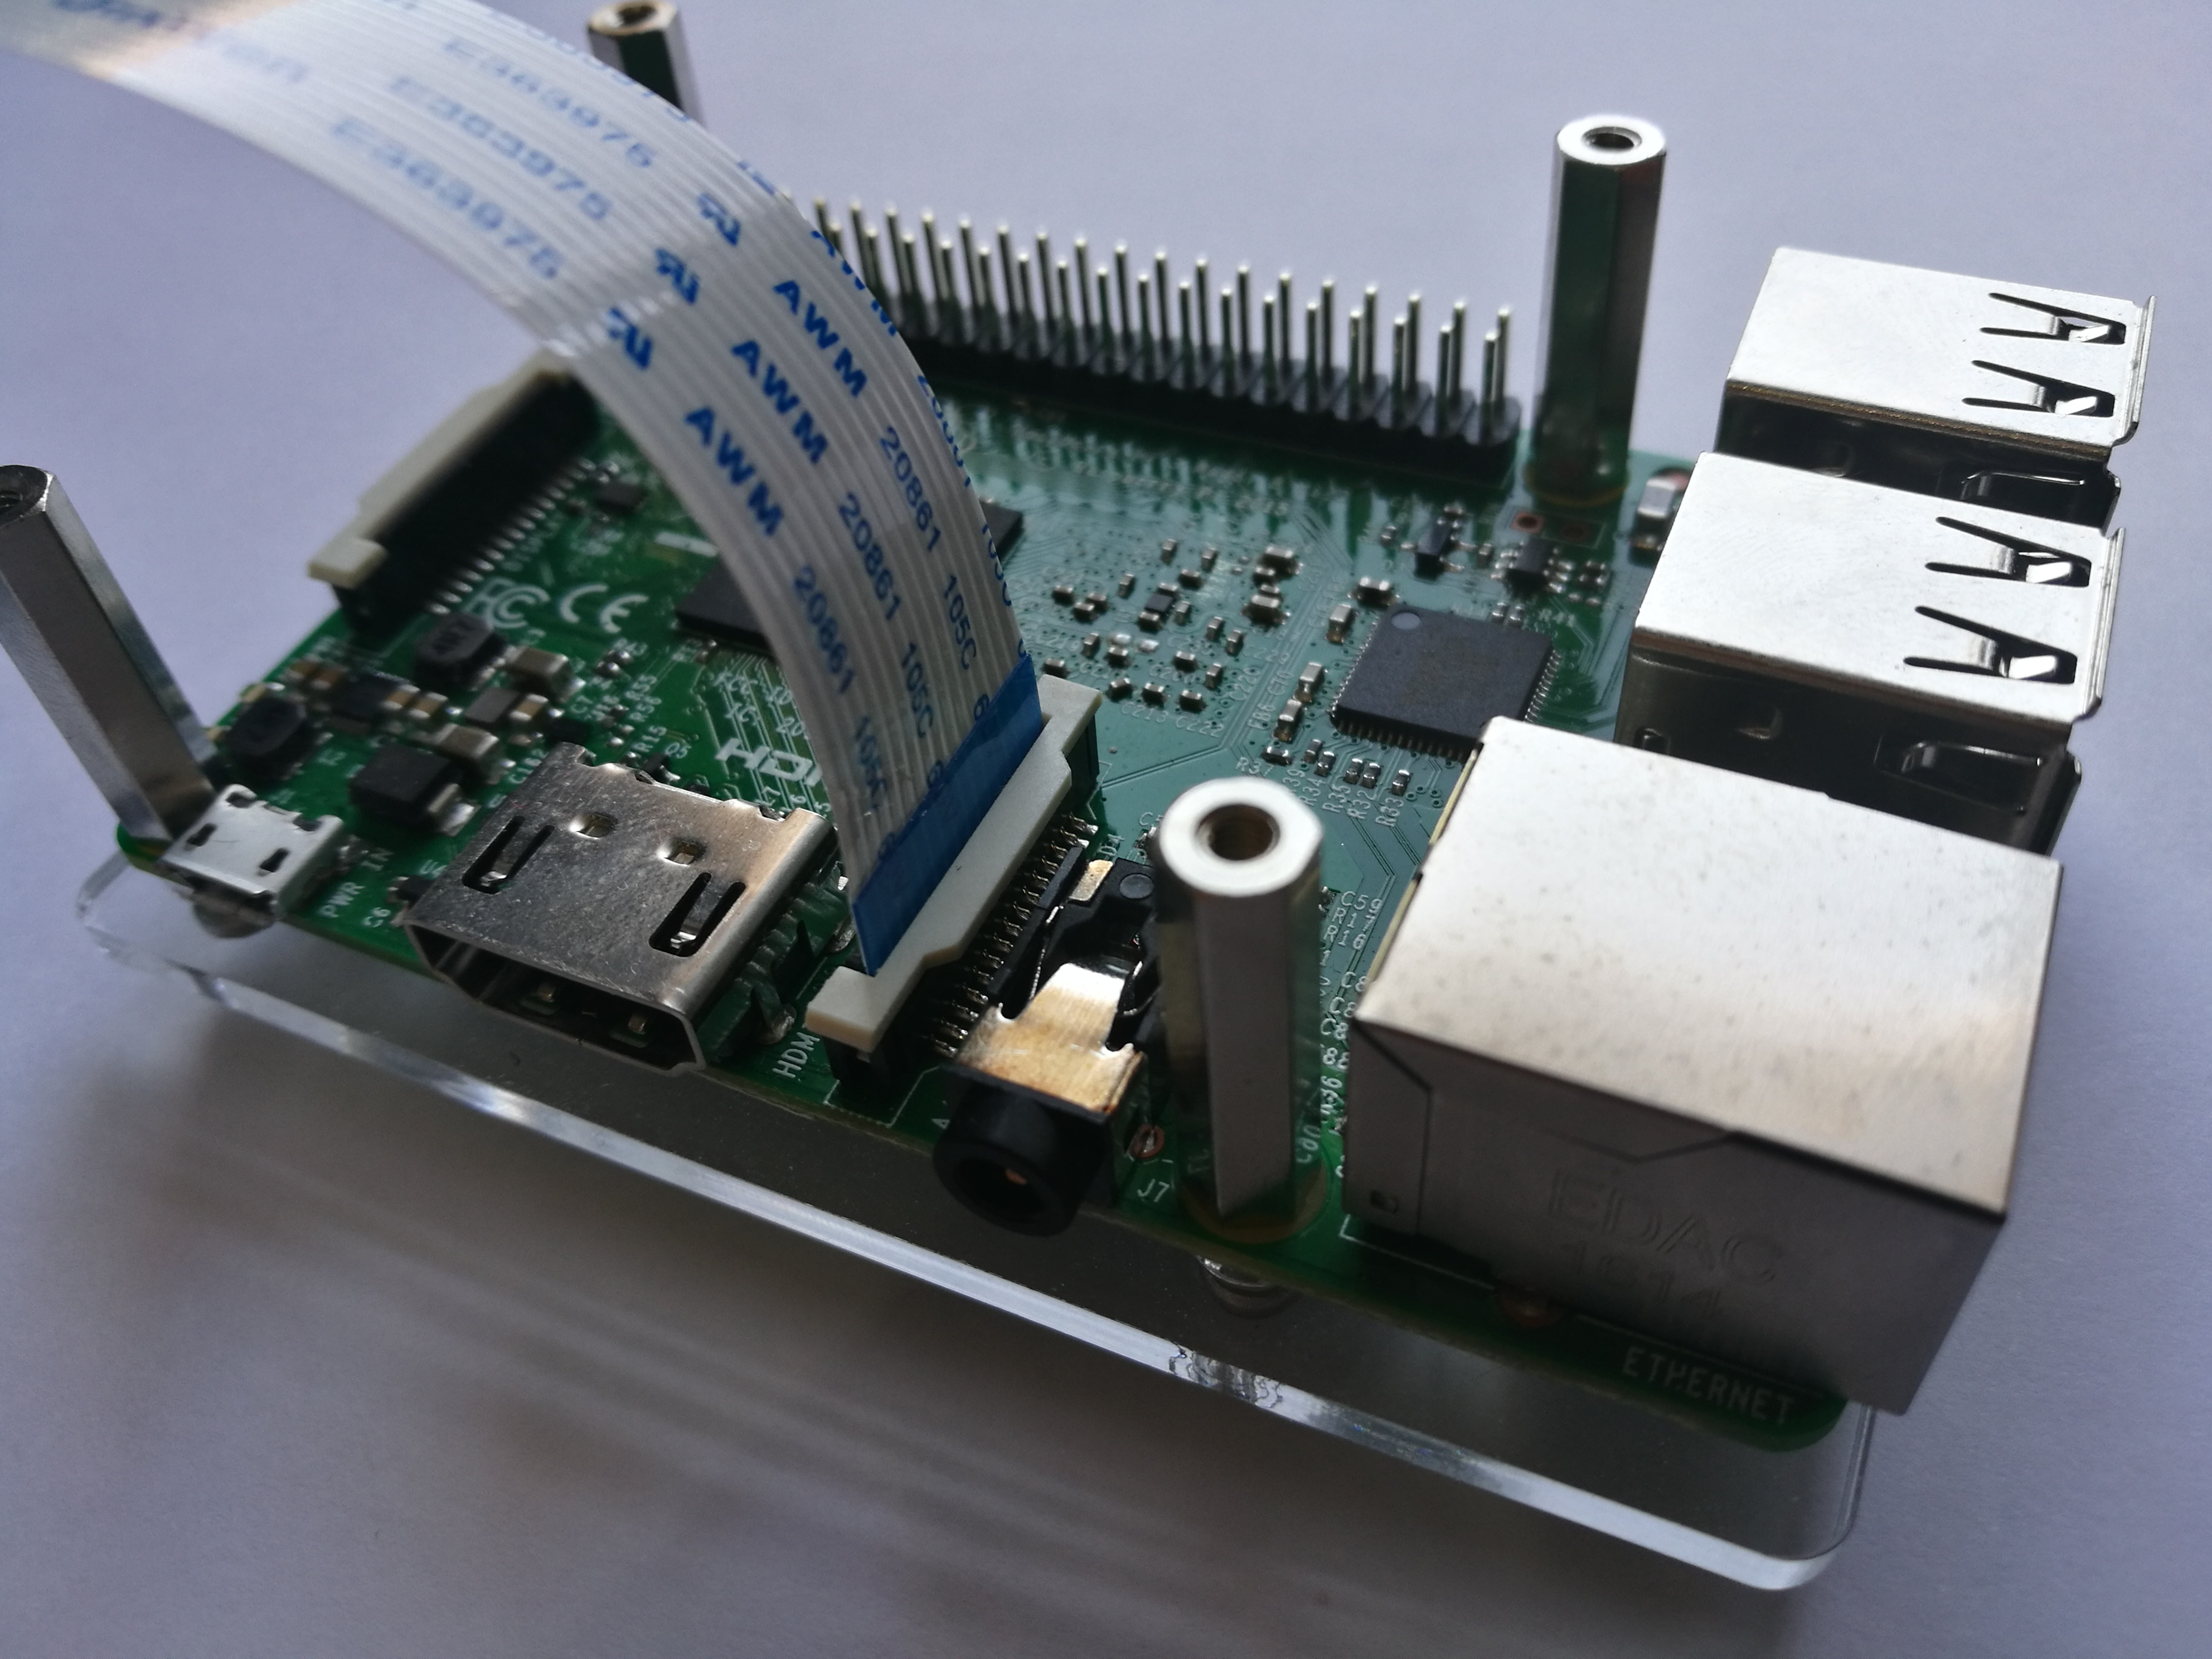
\includegraphics[width=0.75\textwidth]{Appendix_camera_conection.jpg}
		\caption{Connection of the camera module to the Raspberry Pi 3.}
		\label{fig:Appendix_camera_conection}
	\end{center}
\end{figure} %TODO: Cambiar imagen ?


\subsection{Installation of the sense hat}
The installation of the sense hat is explained on Task T2.4.1 of the Sprint 2 on the  \nameref{chap:results} chapter.

\subsection{Installation of the sensors}
The installation of the sense hat is explained on Tasks T2.4.2 and T2.5.1 of the Sprint 2 on the  \nameref{chap:results} chapter.


\subsection{Installation of the necessary libraries}
Some libraries are needed in order to execute the software developed in this \ac{BSc.} thesis:
\begin{enumerate}
	\item NumPy. Is the fundamental package for scientific computing with Python. NumPy can also be used as an efficient multi-dimensional container of generic data. To install it, the next command has to be executed:
\begin{console}
$ sudo apt-get install python-numpy python3-numpy
\end{console} %$

	\item Matplotlib. Is a library for the generation of graphic from data contained in list or arrays using Python programming language and the NymPy package. It provides a MATLAB-like interface. To install it, the next command has to be executed:
\begin{console}
$ sudo apt-get install python-matplotlib python3-matplotlib
\end{console} %$

	\item MP4Box. It can be used for performing many manipulations on multimedia files like AVI, MPG, TS, but mostly on ISO media files (e.g. MP4, 3GP). The justification for using it is that PiCamera generates the video recordings in \emph{h265} format. Therefore, this tool is used to convert videos from \emph{h265} to \emph{mp4}. The installation is done by executing the command:
\begin{console}
$ sudo apt-get install gpac
\end{console} %$
	Once installed, any video (named \texttt{video.h264}) can be converted from \emph{h265} to \emph{mp4} at 30 \ac{FPS} using:
\begin{console}
$ MP4Box -fps 30 -add video.h264 video.mp4
\end{console} %$

	\item Sense hat. To allow Raspberry Pi access the Sense Hat module, the corresponding library has to be installed:
\begin{console}
	$ sudo apt-get install sense-hat
\end{console} %$

	\item IBM Watson \ac{IoT} Platform. Some libraries are needed to allow Python to use the IBM Watson \ac{IoT} Platform services, which are used to send the sensor data to the Cloud. These libraries can be installed by executing the following commands:
\begin{console}
	$ sudo pip3 install ibmiotf
\end{console} %$

\end{enumerate}

When all these steps are completed, the Raspberry Pi is prepared for the correct execution of the software developed in this \ac{BSc.} thesis.
